\documentclass{article}
\usepackage[utf8]{inputenc}
\usepackage[spanish]{babel}
\usepackage{amsmath}
\usepackage{amsfonts}
\usepackage{amssymb}
\usepackage{graphicx}
\usepackage{geometry}

\geometry{a4paper, margin=1in}

\title{Análisis de Elementos de Entrada y Salida del Sistema WorkCodile}
% \author{Gemini CLI Agent}
\date{\today}

\begin{document}
	\maketitle

	\section*{Introducción}
	Este documento detalla los elementos de entrada y salida del sistema
	WorkCodile, centrándose específicamente en las interacciones a nivel de la interfaz
	de usuario (UI). Se identifican los puntos donde el sistema recibe información
	del usuario y donde presenta información al usuario.

	\section*{I. Entradas del Sistema (a través de la Interfaz de Usuario)}
	Estos son los elementos de la UI donde el usuario proporciona información o
	interactúa con la aplicación.

	\subsection*{A. Autenticación y Gestión de Cuenta}
	\begin{itemize}
		\item \textbf{Campos de Texto (Input)}: Para correo electrónico, nombre de
			usuario, contraseña (en \texttt{AuthPage}, \texttt{Settings}).
			\begin{center}
				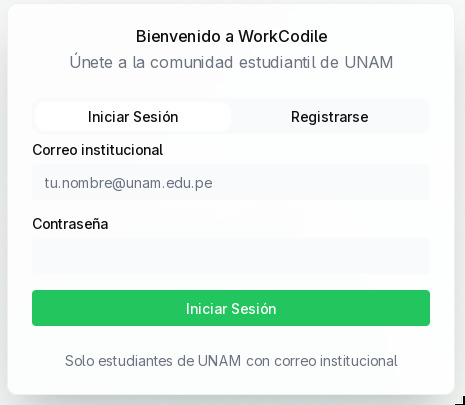
\includegraphics[width=0.4\textwidth]{img/01.jpg}
			\end{center}

		\item \textbf{Botones (Button)}: Iniciar Sesión", "Registrarse", "Recuperar Contraseña",
			"Guardar Cambios", "Cambiar Contraseña", "Eliminar Cuenta".

		\item \textbf{Casillas de Verificación (Checkbox)}: "Recordarme".

		\item \textbf{Campos de Subida de Archivos (Input type="file")}: Para imagen
			de perfil (en \texttt{Settings}).
	\end{itemize}

	\subsection*{B. Creación y Gestión de Contenido}
	\begin{itemize}
		\item \textbf{Campos de Texto (Input)}: Para título de la publicación,
			etiquetas (en \texttt{CreatePostModal}).

		\item \textbf{Áreas de Texto (Textarea)}: Para cuerpo de la publicación,
			contenido del comentario (en \texttt{CreatePostModal}, \texttt{SinglePostView}).

		\item \textbf{Campos de Subida de Archivos (Input type="file")}: Para adjuntos
			de publicación (en \texttt{CreatePostModal}).

		\item \textbf{Botones (Button)}: "Publicar", "Guardar Borrador", "Cancelar",
			"Enviar Comentario", "Editar", "Eliminar".
	\end{itemize}

	\subsection*{C. Interacción con Contenido Existente}
	\begin{itemize}
		\item \textbf{Botones (Button)}: "Me gusta/Votar", "Comentar", "Compartir",
			"Reportar", "Responder", "Votar arriba", "Votar abajo" (en \texttt{PostCard},
			\texttt{Comment}, \texttt{PostActions}).

		\item \textbf{Clics en Elementos de Contenido}: En títulos de publicaciones,
			cuerpos de comentarios, perfiles de usuario para navegar o expandir información.
	\end{itemize}

	\subsection*{D. Navegación y Filtrado}
	\begin{itemize}
		\item \textbf{Campos de Texto (Input)}: Barra de búsqueda (en \texttt{Header}).

		\item \textbf{Botones/Enlaces (Button/Link)}: Elementos de menú de navegación,
			categorías, temas, enlaces rápidos (en \texttt{Header}, \texttt{Sidebar}, \texttt{RightSidebar}).

		\item \textbf{Selectores (Select)}: Para opciones de filtrado (en \texttt{Sidebar},
			\texttt{MobileCourseFilter}).

		\item \textbf{Casillas de Verificación (Checkbox)}: Para aplicar filtros.

		\item \textbf{Desplazamiento (Scroll)}: Para cargar más contenido (paginación
			infinita en \texttt{MainFeed}).
	\end{itemize}

	\subsection*{E. Interacciones Genéricas de UI}
	\begin{itemize}
		\item \textbf{Controles Deslizantes (Slider)}: Para seleccionar valores en un
			rango.

		\item \textbf{Selectores de Fecha (Calendar)}: Para seleccionar fechas.

		\item \textbf{Interruptores (Switch)}: Para activar/desactivar opciones.
	\end{itemize}

	\section*{II. Salidas del Sistema (a la Interfaz de Usuario)}
	Estos son los elementos de la UI donde el sistema presenta información o retroalimentación
	al usuario.

	\subsection*{A. Visualización de Contenido Principal}
	\begin{itemize}
		\item \textbf{Listas de Publicaciones}: Muestra \texttt{PostCard}s con título,
			autor, extracto, metadatos (en \texttt{MainFeed}).

		\item \textbf{Detalles de Publicación}: Título, cuerpo completo, archivos adjuntos,
			autor, fecha (en \texttt{SinglePostView}).

		\item \textbf{Árbol de Comentarios}: Comentarios anidados con autor,
			contenido, fecha (en \texttt{CommentTree}).

		\item \textbf{Perfiles de Usuario}: Nombre de usuario, imagen de perfil, biografía,
			estadísticas, publicaciones (en \texttt{UserProfile}).

		\item \textbf{Secciones Dinámicas}: \texttt{TrendingSection} (temas/publicaciones
			populares), \texttt{RecentActivity} (actividad reciente).

		\item \textbf{Logros}: Insignias, progreso, notificaciones de logros (en
			\texttt{AchievementSystem}).
	\end{itemize}

	\subsection*{B. Retroalimentación y Notificaciones}
	\begin{itemize}
		\item \textbf{Mensajes de Notificación (Toaster)}: Mensajes emergentes de éxito,
			error, información.

		\item \textbf{Panel de Notificaciones}: Lista de notificaciones (en \texttt{NotificationsPanel},
			\texttt{EnhancedNotifications}).

		\item \textbf{Indicadores de Carga}: Spinners, esqueletos de contenido (en \texttt{LoadingComponents}).

		\item \textbf{Mensajes de Error/Validación}: Retroalimentación en formularios
			sobre entradas no válidas o errores de procesamiento.

		\item \textbf{Cambios de Estado Visual}: Botones deshabilitados, campos
			resaltados.
	\end{itemize}

	\subsection*{C. Elementos de Navegación y Estado}
	\begin{itemize}
		\item \textbf{Encabezado}: Avatar del usuario, nombre de usuario, enlaces de
			navegación, resultados de búsqueda (en \texttt{Header}).

		\item \textbf{Barras Laterales}: Enlaces de navegación, filtros activos, información
			contextual (en \texttt{Sidebar}, \texttt{RightSidebar}).

		\item \textbf{Estado de Autenticación}: Mostrar avatar/nombre de usuario o botones
			de inicio de sesión/registro.

		\item \textbf{Contadores}: Número de "Me gusta", comentarios, notificaciones.
	\end{itemize}

	\subsection*{D. Elementos Visuales y Estilísticos}
	\begin{itemize}
		\item \textbf{Diseño General}: Aplicación de estilos y temas (colores, tipografía).

		\item \textbf{Efectos Visuales}: Animaciones de fondo, efectos de
			glassmorphism (\texttt{GlassCard}), efectos de hover, sombras.

		\item \textbf{Iconos y Calificaciones}: \texttt{CrocodileIcon}, \texttt{CrocodileRating}.
	\end{itemize}
\end{document}